\section{The KLFitter} \label{sec:KLFitter} 

In order to validate the effectiveness of the top reconstruction BDT, we test its performance against that of the Kinematic Likelihood Fitter (KLFitter) \ref{cite:KLFitter}. 

The KLFitter is a likelihood-based framework that, like the BDT, attempts to solve the top reconstruction combinatorial jet-matching problem. To correctly identify the jet triplet originating from the top, the KLFitter maximizes a likelihood function that depends on the kinematics of each of the final-state jets for each possible jet permutation. Based on this likelihood-maximization, an event probability is calculated that allows us to identify the best potential top candidate from the jet permutations.

For semileptonic tops (the decay mode in which we perform this study), the form of the likelihood function is:

\begin{flalign}
\begin{aligned}
\mathcal{L} = \mathcal{B}(m_{q_{1}q_{2}q_{3}} | m_{t}, \Gamma_{t}) \times \mathcal{B}(m_{q_{1}q_{2}} | m_{W}, \Gamma_{W}) \times \\
\mathcal{B}(m_{q_{4}l\nu} | m_{t}, \Gamma_{t})  \times \mathcal{B}(m_{l\nu} | m_{W}, \Gamma_{W}) \times \\
\prod_{i=1}^{\infty} C_{jet}(E_{jet,i}^{meas}|E_{jet,i}) \times C_{l}(E_{l}^{meas}|E_{l}) \times \\
C_{miss}(E_{x}^{miss}|p_{x}^{\nu}) \times C_{miss}(E_{y}^{miss}|p_{y}^{\nu})
\end{aligned}
\end{flalign}

where the $\mathcal{B}$s denote Breit-Wigner functions (similar to Gaussians, dependent on both mass and decay width) and the C terms indicate transfer functions, designed to model the difference between measured kinematics and their true values due to detector effects. At the time of this study, transfer functions for the ATLAS detector were defined only for jets with $|\eta|< 4.5$, so we restrict our study to this range.

The log-likelihood algorithm is minimized using the Minuit algorithm \ref{cite:Minuit} as implemented in the Bayesian Analysis Toolkit (BAT) \ref{cite:BAT}.

\begin{figure}
	\centering
	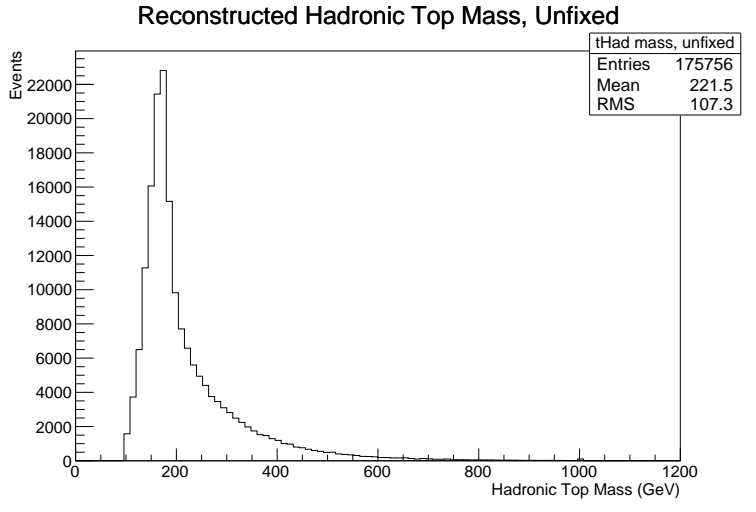
\includegraphics[width=0.31\linewidth]{figures/KLFitter/KLFittertopmass.png}
	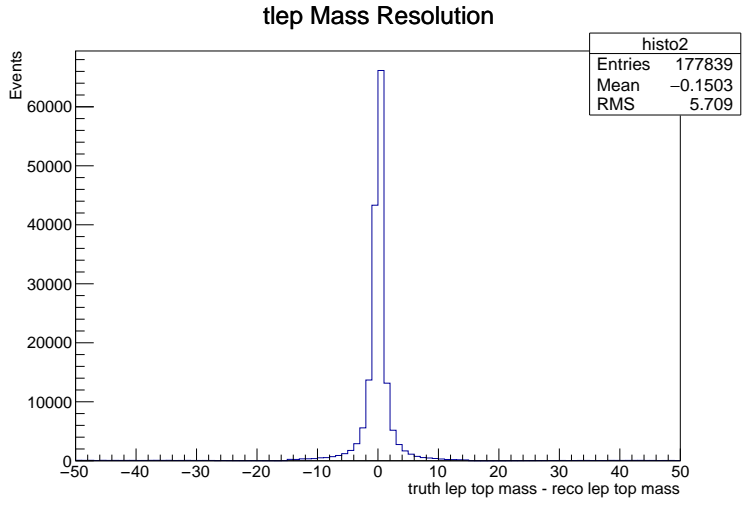
\includegraphics[width=0.31\linewidth]{figures/KLFitter/KLfitter1.png}
	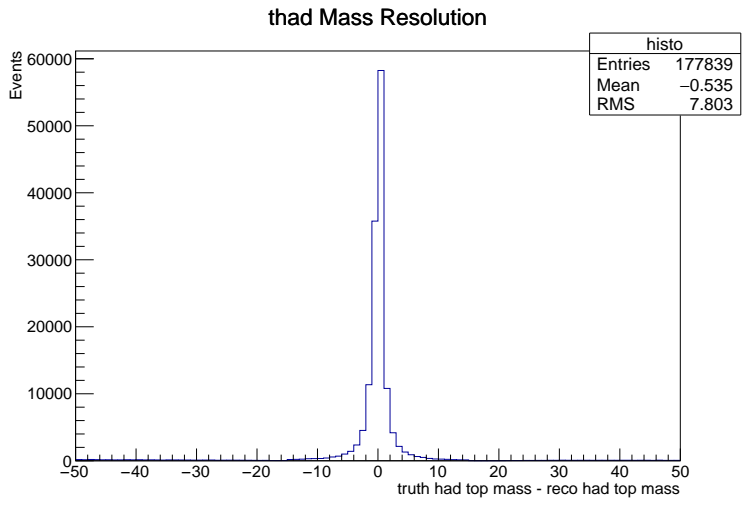
\includegraphics[width=0.31\linewidth]{figures/KLFitter/KLfitter2.png}
	\caption{Reconstructed top-mass and top-mass resolution of the KLFitter (using the "unfixed" top-mass setting to illustrate performance).}
	\label{fig:sel_topReco_retrain}
\end{figure}

\section{Comparison} \label{sec:comparison} 

In order to compare the KLFitter and BDT methods, we construct a validation set of truth-tagged semileptonic top events. We use the "mc16a" (2015-like pileup profile) PowhegPy8 $ttH$ sample, and select only events which contain at least four jets and exactly one lepton, all with $|\eta|< 4.5$.

We find that KLFitter performs optimally when we fix the top mass to its measured value of 172.5 GeV \ref{cite:topmass} and use the 'kWorkingPoint' b-tag handling method, which adds an additional multiplier to the event probability to account for the b-tagging efficiency and light-jet rejection. 

\begin{table}[h]
    \centering
    \begin{tabular}{|c|c|c|c|}
    \hline
    & Correct Leptonic Tops (\%) & Correct Hadronic Tops (\%) & Both Correct (\%) \\ \hline
    KLFitter & 55.59 & 21.92 & 16.20 \\ \hline
    Top Reco BDT & 60.19 & 21.35 & 17.92 \\ \hline   	
    \end{tabular}
    \caption{Comparison of KLFitter and top-reconstruction BDT.}
    \label{KLFitterTable}
\end{table}
